%TODO once the text is "finished": Figure out first appearance of all words in the glossary and make sure that the first mention of it is written out with the abbreviation in parantheses
\documentclass[11pt,
  paper=a4, 
  bibliography=totocnumbered,
	captions=tableheading,
	BCOR=10mm
]{scrreprt}

\usepackage[utf8]{inputenc}
 
 
\usepackage[onehalfspacing]{setspace}
\usepackage{csquotes} % Context sensitive quotation.
\usepackage{amsmath} % Standard math.
\usepackage{amsthm} % Math theorems.
\usepackage{amssymb} % More math symbols.
\usepackage{dsfont} % Render |R and the like
\theoremstyle{definition}
\newtheorem{definition}{Definition}[chapter]
 
\usepackage{url}
\usepackage[section]{placeins} % Keep floats in the section they were defined in.
\usepackage{tabularx}
\usepackage{booktabs} % Scientific table styling.
\usepackage{floatrow} % Option for keeping floats in the place they were defined in the code.
\floatsetup[table]{style=plaintop}
\usepackage{hyperref} % Hyperlinks.
\usepackage[all]{nowidow} % Prevent widows and orphans.
\usepackage{xstring} % logic string operations
\usepackage{bbm} % \mathbb on numerals.
\usepackage{csquotes}
\usepackage{mathtools}
\usepackage[ruled,vlined]{algorithm2e} % Pseudocode
\usepackage{scrhack} % Make warning go away.
\usepackage{graphicx}
\usepackage{subcaption} % Subfigures with subcaptions.
\usepackage{authoraftertitle} % Make author, etc., available after \maketitle
\usepackage{listofitems}
\usepackage{blindtext} % Placeholder text.
\usepackage[automake, nopostdot, nonumberlist]{glossaries} % glossary for definitions and acronyms, without dot after entry and page reference 
\makeglossaries % Generate the glossary

% \PassOptionsToPackage{obeyspaces}{url}%
\usepackage[backend=bibtex,% 
style=nature,% 
doi=true,isbn=false,url=false, eprint=false]{biblatex}
% \renewbibmacro*{url}{\printfield{urlraw}}

\addbibresource{mendeley_bibs/Masterarbeit.bib}

\DeclareStyleSourcemap{
  \maps[datatype=bibtex, overwrite=true]{
    \map{
      \step[fieldsource=url, final]
      \step[typesource=misc, typetarget=online]
    }
    \map{
      \step[typesource=misc, typetarget=patent, final]
      \step[fieldsource=institution, final]
      \step[fieldset=holder, origfieldval]
    }
  }
}

%\linespread{1.5} % set line spacing
 
\usepackage{listings} % rendering program code
\lstset{% general command to set parameter(s)
	basicstyle=\ttfamily\color{grey},          % print whole listing small
	keywordstyle=\color{black}\bfseries\underbar,
	% underlined bold black keywords
	identifierstyle=,           % nothing happens
	commentstyle=\color{white}, % white comments
	stringstyle=\ttfamily,      % typewriter type for strings
	showstringspaces=false}     % no special string spaces


\DeclareFontFamily{U}{mathx}{\hyphenchar\font45}
\DeclareFontShape{U}{mathx}{m}{n}{
      <5> <6> <7> <8> <9> <10>
      <10.95> <12> <14.4> <17.28> <20.74> <24.88>
      mathx10
      }{}
\DeclareSymbolFont{mathx}{U}{mathx}{m}{n}
\DeclareFontSubstitution{U}{mathx}{m}{n}
\DeclareMathSymbol{\bigtimes}{1}{mathx}{"91}

 

%%% Custom definitions %%%
% Shorthands
\newcommand{\ie}{i.\,e.~}
\newcommand{\eg}{e.\,g.~}
\newcommand{\ind}{\mathbbm{1}}
% Functions
\newcommand{\tpow}[1]{\cdot 10^{#1}}
\newcommand{\figref}[1]{(Figure \ref{#1})}
\newcommand{\figureref}[1]{Figure \ref{#1}}
\newcommand{\tabref}[1]{(Table \ref{#1})}
\newcommand{\tableref}[1]{Table \ref{#1}}
\newcommand{\secref}[1]{%
	\IfBeginWith{#1}{chap:}{%
		(cf. Chapter \ref{#1})}%
		{(cf. Section \ref{#1})}%
		}
\newcommand{\sectionref}[1]{%
	\IfBeginWith{#1}{chap:}{%
		Chapter \ref{#1}}%
		{\IfBeginWith{#1}{s}{%
			Section \ref{#1}}%
			{[\PackageError{sectionref}{Undefined option to sectionref: #1}{}]}}}
\newcommand{\chapref}[1]{(see chapter \ref{#1})}
\newcommand{\unit}[1]{\,\mathrm{#1}}
\newcommand{\unitfrac}[2]{\,\mathrm{\frac{#1}{#2}}}
\newcommand{\codeil}[1]{\lstinline{#1}}{} % wrapper for preventing syntax highlight error
\newcommand{\techil}[1]{\texttt{#1}}
\newcommand{\Set}[2]{%
  \{\, #1 \mid #2 \, \}%
}
% Line for signature.
\newcommand{\namesigdate}[1][5cm]{%
	\vspace{5cm}
	{\setlength{\parindent}{0cm}
	\begin{minipage}{0.3\textwidth}
		\hrule 
		\vspace{0.5cm}
		{\small city, date}
	\end{minipage}
	 \hfill
	\begin{minipage}{0.3\textwidth}
		\hrule
		\vspace{0.5cm}
	    {\small signature}
	\end{minipage}
	}
}
% Automatically use the first sentence in a caption as the short caption.
\newcommand\slcaption[1]{\setsepchar{.}\readlist*\pdots{#1}\caption[{\pdots[1].}]{#1}}

% Variables. 
% Adapt if necessary, use to refer to figures and graphics.
\def \figwidth {0.9\linewidth}
\graphicspath{ {./graphics/figures/}{./graphics/figures/} } % Path to figures and images.


% Customizations of existing commands.
\renewcommand{\vec}[1]{\mathbf{#1}}
% Capitalized \autoref names.
\renewcommand*{\chapterautorefname}{Chapter}
\renewcommand*{\sectionautorefname}{Section}


% TODO Fill with your data.
\title{Data-Driven Embedding of educational resources in a vector-space with interpretable Dimensions for Explainable Recommendation}
\author{Christoph Stenkamp}

\begin{document}

\begin{titlepage}
	\begin{flushleft}
		Universität Osnabrück\\
		Fachbereich Humanwissenschaften\\
		Institute of Cognitive Science
	\end{flushleft}

	\vspace{2cm}
	\centering{
		Master's thesis\vspace{1cm}\\
		\textbf{\Large{\MyTitle}}
		\vspace{1cm}\\
		\begin{tabular}{c}
			\MyAuthor                          \\
			955004                             \\
			Master's Program Cognitive Science \\
			April 2017 - February 2022
		\end{tabular}}
	\vspace{1cm}

	\begin{tabular}{ll}
		First supervisor:  & Dr. Tobias Thelen          \\
		                   & Institute of Cognitive Science \\
		                   & University of Osnabrück  \\\\
		Second supervisor: & Johannes Schrumpf, M.Sc.         \\
		                   & Institute of Cognitive Science \\
		                   & Osnabrück
	\end{tabular}

\end{titlepage}


\chapter*{Declaration of Authorship}
I hereby certify that the work presented here is, to the best of my knowledge and belief, original and the result of my own investigations, except as acknowledged, and has not been submitted, either in part or whole, for a degree at this or any other university.

\namesigdate
\pagenumbering{gobble}
\pagebreak

\begin{abstract}
	\textbf{\LARGE{Abstract}}\\\\
	%TODO summarize the main objectives and outcomes of your work. The abstract should fit on one page.
	In this thesis, I want to generate a conceptual space for the domain of educational reasources such as university courses, automatically created in data-driven way from their descriptions.

	Conceptual Spaces are seen as something that may be able to link sub-symbolic and symbolic approaches by standing in between them: In Conceptual Spaces, Concepts are represented as convex regions in high-dimensional spaces. Optimally, these spaces are cartesian, and the axes correspond to human-interpretable dimensions. If that is the case, you could for example classify the concept of "Apple" as a region that is in the color-dimension somwhere between green and red, and in the form-dimension roughly at "round".
	Creating these concpetual spaces is a very cumbersome task, which is why an automated method may lead to reasonable results. Unfortunately, this is still computationally very complex.
	The method of [DESC15] uses MDS, blablabla, then a Support-Vector-Machine separating concepts, and the orthogonal of the separating hyperplane is then an axis
\end{abstract}




\tableofcontents
\listoffigures
\listoftables
\listofalgorithms


\chapter{Introduction}
\pagenumbering{arabic}

% Broad - "Initialkontextualisierung" - warum mach ich das, aus was für ner domain kommen die daten, was will ich damit machen (use rrecommendation, ich bau AI part, ..)

In this thesis, I want to generate a conceptual space for the domain of university courses, automatically created in data-driven way from their descriptions.

\section{What are conceptual spaces? }

Conceptual spaces (Gärdenfors, blabla) want to stand in between subsymbolic processing and symbolic processing: Like in subsymbolism, concepts are represented in high-dimensional spaces, but because the dimensions of these spaces are not arbitrary but human-interpretable, it allows for symbolistic high-level reasoning.

So, in conceptual spaces, concepts are represented as convex regions in high-dimensional, human interpretable spaces. For example, the concept of "apple" is a region that in the dimension "color" is somewhere between red and green, in the dimension "form" at roughly round, in the dimension "taste" somwhere between sweet and sour, etc. 
Every instance of an apple is thus a vector that lies inside the high-dimensional region of the concept. This allows for high-level reasoning, such as the question "does any Instance of concept X fit into my bag?" -> If the "size" dimension of the whole region is smaller than the size of my bag, it will.

Conceptual spaces sounds similar to word2vec or other word embedding approaches, however there are a few important distinctions - first, the domain of a conceptual space does not include all kinds of words or concepts, but only concepts of a certain domain (like movies or university courses). 
Second, conceptual spaces are convex regions, not mere vectors (which allows for easy extraction of is-a and part-of relations or prototypical examples vs edge examples, but makes the generation computationally vastly more expensive). And, most importantly, while the geometry of word2vec is roughly euclidian (otherwise the famous vec(king)-vec(man)+vec(woman)==vec(queen) wouldn't work), the dimensions are not interpretable but arbitrarily depend on the random initial setup, so the concepts king and queen differ not only in a single "gender" dimension [..and also its not really euclidian, is it?! sonst wäre die betweeness doch nicht so special, oder?].

Now the standard problem with conceptual spaces is that they would have to be manually generated, which of courses is a lot of work, which is where the work of [Schokeart et al] comes in - to generate them in a data-driven fashion.
For that, the authors look at three different domains: movies, wines and places. For each of these domains, they collected many samples (like movies) together with descriptions from places where people can leave them (like reviews from IMDB). A representation of a movie is then generated from the bag-of-words of the descriptions of the individual movies, leading to a very high-dimensional, very sparse representation for all movies. 
To make the representations less sparse and more meaningful, the words in the BOW are subsequently PPMI-weighted, which weights words that appear often in the description of a particular movie while being infrequent in the corpus overall higher while setting the representation of stopwords to almost zero. 
This PPMI-weighted BOW is however not yet a euclidian space yet, which is why the authors subsequently use multidimensional scaling (MDS). MDS is a diminsionality reduction technique that attempts to create a euclidian space of lower dimensionality than the original one in which the individual distances of the items are preserved as well as possible. 

With such a space, the concepts of betweeness already makes sense, but so far, the dimensions are not interpretable. So how does one automatically find such directions? In the case of movies, good dimensions may be "scariness", "funniness", "epicness", "family-friendlyness" etc. 
To find these dimensions, the authors look for these words (as well as similar words thanks to clustering) in the reviews. Then the movies are grouped into those that contain the words from the cluster often enough vs those that don't. A support-vector-machine subsquently finds a hyperplane that best divides the two groups (eg. scary and non-scary), and the orthogonal of that hyperplane is used as one axis of the new coordinate basis. 

% TODO: Ist word2vec schon nen euclidian space? Why/Why not?

% \begin{figure}[H]
% 	\centering
% 	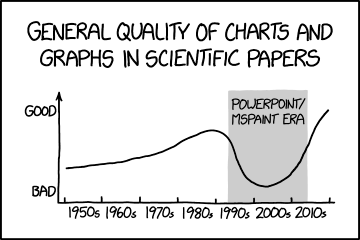
\includegraphics[width=\figwidth]{scientific_paper_graph_quality}
% 	\slcaption{
% 		Developmemt of scientific paper graph quality. A dip in the
% 		quality of scientific graphs is observed from the early 1990s to the early 2010s.
% 		During this time Microsoft Paint and PowerPoint were often used to create graphs in scientific papers.\label{fig:scientific_graph_quality}}
% \end{figure}

% \begin{table}[H]
% 	\begin{tabular}{@{}ll@{}}
% 		\toprule
% 		year & quality \\ \midrule
% 		1985 & good    \\
% 		2000 & bad     \\ \midrule
% 		2015 & better  \\ \bottomrule
% 	\end{tabular}
% 	\caption{
% 		Empirical measurements of scientific graph quality. Data points were collected using
% 		a systematic literature review.\label{tab:scientific_graph_quality}}
% \end{table}
% This references a \figref{fig:scientific_graph_quality} while this references a table \tabref{tab:scientific_graph_quality}.

% A citation looks like this \cite{hadash2018estimate}. To embed a citation in the text flow use textcite,
% \eg \textcite{hadash2018estimate} said you should use a lot of citations.

\chapter{Theoretical Background}
% (zuspitzung von generell auf spezifisch, sowohl technisch (conceputalspaces -> was macht das paper konkret), (und bei dem anderen teil was sind educational resources, was sind die schwierigkeiten dabei, warum möchte man überhaupt empfehlen))

\section{Use Case: Educaional Resources}
% Anwendungsfall (->e-learning, recommenden von bildungsressourcen, ...) -> nicht-technisch, aber nötig zum verstehen wo passiert das 

\section{Conceptual Spaces}

\section{Automatic Data-Driven Generation of Conceptual Spaces}
%Wie funktioniert die Idee des data-driven generieren 

\chapter{Methods}
%(Algorithmus & Datensatz)

\section{Dataset}
% Empirie, auch specifics über den Datensatz

%To write:
% * where does the data come from
% * what size is the data, what is the distribution, ...
% * Preliminary analysis (if I delete all that are shorter than X, it are |Y|..)
% * Does it cluster and look nice?
% * Verteilung der Sprachen
% * Preprocessing in kurzem Fließtext beschreiben - "After throwing out all descriptions shorter than xyz chars, 2323 courses where left. 223 of these were ..."


The main goal of this thesis was to create a conceptual space of courses, automatically generated by course descriptions.


For that, a dataset of courses and their descriptions was obtained as export from the Stud.IP system as used at the universities of Osnabrück, Hannover and Bremen.
%TODO wait, woher kam der datensatz überhaupt? Tobias hat mir den geschickt, aber kam er zustande im Rahmen von Siddata?


\begin{figure}[H]
	\centering
	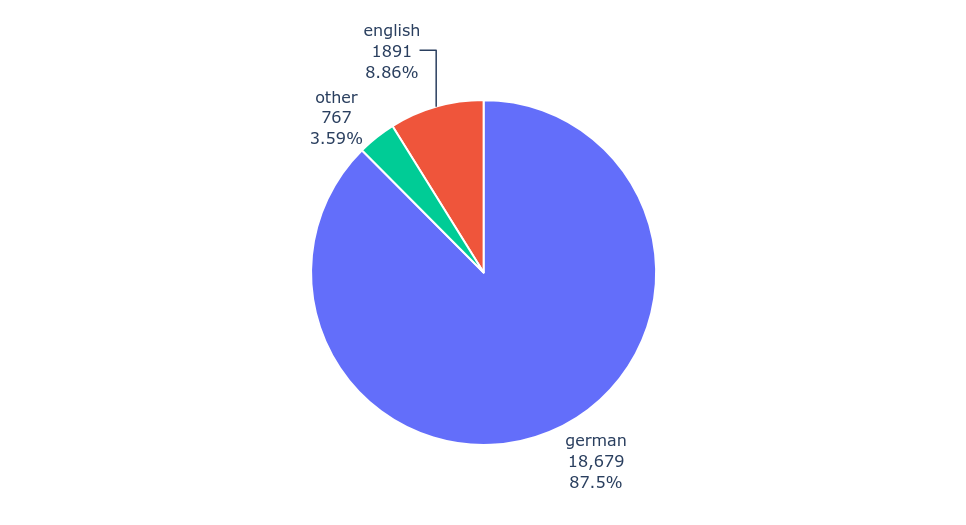
\includegraphics[width=\figwidth]{graphics/figures/courses_language_distribution.png}
	\slcaption{
		\label{fig:courses_language_distribution}
		Distribution of languages of course descriptions.
		%TODO figure if this is the correct amount of preprocessing/throwout to have done
		Of the 21337 courses left after preprocessing, 18,679 were in german language according to the \textit{langdetect} python-package\footnote{\url{https://pypi.org/project/langdetect/}, which is a direct port of a java library\ which claims to have 99.8\% accuracy on longer texts\cite{nakatani2010langdetect}}.
		}
\end{figure}

To see if it is possible to extract any kind of structured data from the unstructured course descriptions, a Neural Network classifier was trained on the dataset, classifying courses to the faculty they run under. 
The faculty is easily obtainable from the dataset, as the first one or two digits of the course ID correspond to it. The distribution of the faculties is depicted in figure \ref{fig:faculty_plot}.

\begin{figure}[H]
	\centering
	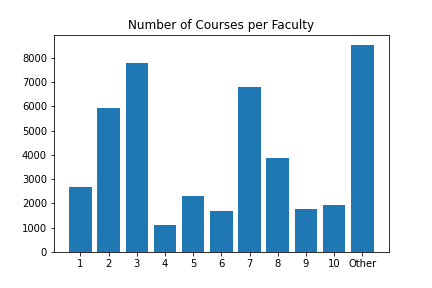
\includegraphics[width=\figwidth]{graphics/figures/faculty_plot.png}
	\slcaption{
		\label{fig:faculty_plot}
		Distribution of faculties in the courses
		}
\end{figure}

The purpose of the Neural Network classifier is to check if it is anyhow possible to extract meaningful information from the descriptions: If it is possible to train a classifier on the data that can reasonably predict a qualitative feature, there is enough structure in the data such that the algorithm I'm about to produce can work.
Also, we have a lower bound for useful data: we can just throw away data that cannot be classified!
%TODO train a second classifier on something else and throw away data that gets classified by neither and inspect it


\section{Algorithm}
%Was für Schritte hat der Algo 

%TODO something along the lines of "Da, based on [source die die accuracy von dem gtranslate algorithm mit denen von menschen vergleicht], a gtranslate translation is as good as the average lecturer, it is assumed that translating the texts to english before using an english model can lead to better results

\subsection{Extracting Candidate Terms}
\label{sec:extract_candidates}

* KeyBERT

%TODO theoretisch ist es auch möglich bspw nen network mit attention auf gewisse dinge wie fachbereich und anderes zu trainieren und dann rauszusuchen was die wichtigen ausschlaggebenden dinge für das Netzwerk waren

%TODO extract using TF/IDF as well

%TODO a source: https://github.com/MaartenGr/KeyBERT#citation

* After you figure out which candidate term appears in which texts, figure out which other terms are frequent in these texts while infrequent in texts of the other class and then add these to the candidate-term-set (other way may even be to classify the texts according to if the candidateterm appears in them, and then take the misclassified one also as positive samples)

\subsection{Calculating the distance to the SVMs Separatrix}
\label{sec:calculate_distance}

%TODO: before this, explain 
% * extraction of the candidate term set
% * how vectors are made from texts
In order to tell how much a text is prototypical of a category, all texts are split depending on whether they contain words of a set as described in \ref{sec:extract_candidates}, before a linear Support Vector Machine Classifier is trained on the vector-representation of all of the texts, splitting them into two classes: those that contain one of the candidate terms and those that do not. Due to the linear kernel, the SVM finds a hyperplane (\textit{separatrix}) that splits the positive from the negative samples in a way that maximizes the distance between the respective classmembers and the separatrix, using samples close to the margin as \textit{support vectors}. %TODO: what if the data is not linearly seperable?

Following the SVMs logic, one could argue that the further away a sample is from this separatrix, the more prototypical it is of its class. Thus, the distance of a sample to its \textit{orthogonal projection onto the hyperplane} %TODO explain orthogonal projection
may serve as metric for how prototypical a sample is for the respective category. 

Translated into terms relevant to the aim of this thesis, the classes may be those educational resources whose description contains the word "\textit{hard}" as one class vs. those that do not as the other class. Now according to [TODO], one may use the distance of the sample towards the separatrix as a measure of how hard a class is: For all positive samples, a longer distance means a harder class, for all negative samples a longer distance means an easier one, whereas those samples close to the separatrix can be considered average.

\subsubsection*{How to calculate the distance}

%TODO mention that I'm in a cartesian coordinate system
%TODO mention that I'm thinking in euclidian coordinates, see https://en.wikipedia.org/wiki/Plane_(geometry)
\noindent In the following paragraphs, I will visualize how to calculate the orthogonal distance from a sample to the hyperplane exemplary for the case of three-dimensional text-vectors.

Generally, the separatrix splitting positive from negative samples for an $n$-dimensional space $\mathds{R}^n$ is an $n-1$-dimensional subspace (called \textit{hyperplane}), which in the case of $\mathds{R}^3$ corresponds to a plane. 
%https://en.wikipedia.org/wiki/Plane_(geometry)#Representation

The general form of the equation of a plane is given as the following linear equation, where parameters $a, b, c$ and $d$ encode the position of the plane:

\begin{equation}
	\label{eq:general_plane}
	ax + by + cz = d
	%TODO source? mein Tafelwerk? :D
\end{equation}

This reads as "All points $(x,y,z)$ for which \ref{eq:general_plane} holds are on the plane". 

In this representation of the plane, the vector $(a,b,c)$ encodes a normal vector orthogonal to this plane, whereas $d$ serves as intercept, encoding the intersection of plane and normal. (specifically: the perpendicular distance you would need to translate the plane along its normal to have the plane pass through the origin) In higher dimensions, the formula for the hyperplane would become $a_1x_1+a_2x_2+a_3x_3+...+a_nx_n = b$, which means that encoding the hyperplane for a space $\mathds{R}^n$ requires $n+1$ parameters.
% one rough quote in this paragraph from https://stackoverflow.com/a/17661431

%TODO explain that it's not even harder in higher-dimensional spaces
%TODO explain that nicely, in python the separatrix is perfectly specified using the normal and the intercept, so we have everything we need 
%TODO die handschriftlichen notizen aus den beiden notebooks einbauen
%TODO die plots aus dem notebook einbauen

% The distance from any point of this $\mathds{R}^n$ to the hyperplane is then calculated as the length of the vector that is the \textit{orthogonal projection} from that point onto the hyperplane. The orthogonal projection from one vector onto another can be calculated as 

% \begin{equation}
% 	\label{eq:orthogonal_projection}
% 	\hat{\vec{a}} = \frac{\vec{a}\cdot\vec{b}}{\vec{b}\cdot\vec{b}}\cdot\vec{b}
% 	%TODO source https://en.wikipedia.org/wiki/Vector_projection
% \end{equation}

% ...as we however have a plane we want to project to, not a vector, what I wrote here is rather useless, isn't it?


The distance from any point of this $\mathds{R}^n$ to the hyperplane can then be calculated as 
% As... * dist(point, point_projected_onplane)     						 (`project[1,3]_pre`)
%       * abs(trafo(point)[0])     										 (`protoypicality_pre`)
%       * np.dot(plane.normal, point) + plane.d							 (`project2_pre')
% ...normiert sind die alle gleich, aber for some reason differn die um nen multiplicator..?!
% And the projections...:
%       * back_trafo([0, trafo(point)[1], trafo(point)[2]]
% 		* plane.project(point): k = (ax+by+cz+d)/(a²+b²+c²); result = [x-ka, y-kb, z-kc]
%       * point - distance * plane.normal  (...aber nur mit protoypicality_pre als distance! )
% 		...note that second and third are basically equal - both calculate "how much do I need to go into the direction of the orthogonal" and then do so  (point - distance * normal). The difference is that in plane.project the distance is divided by (a²+b²+c²). Originally sagt der typ von SO (https://stackoverflow.com/a/17661431) die distance ist einfach n*p-d, dann fehlt nur der normierungsterm. 
% TODO: figure out the explanation of the difference from this to the result of using forward and backward??
% See get_svm_decisionboundary.ipynb, den kram zwischen `#deleteme from here', commit d46a8300dae81adee





\chapter{Results}


\chapter{Discussion and Conclusion}
% (was sind die broaden takeaways von meinem Kram)
% * Nochmal nen theoretisches Embedding, Kontextualisieren für Bildungsressourcen
% * ...and conclusion


\chapter*{Acknowledgements}
%TODO A place to say thank you to everybody who helped you.


% START Acronym definitions
\newacronym{utc}{UTC}{Universal Time Coordinated}
\newacronym{ml}{ML}{Machine Learning}
\newacronym{svm}{SVM}{Support Vector Machine}
\newacronym{mds}{MDS}{Multi Dimensional Scaling}
\newacronym{ppmi}{PPMI}{Positive Pointwise Mutual Information}
\newacronym{bow}{BOW}{Bag Of Words}
\newacronym{imdb}{IMDB}{Internet Movie Database}
% END Acronym definitions

\glsaddall
\printglossaries %TODO let glossary appear in TOC

\printbibliography

\end{document}
